\documentclass{article}

\usepackage{graphicx}
\usepackage[svgnames]{xcolor}
\usepackage{tikz}
\usepackage{pgfplots}
\usepackage{fontspec}
\usepackage{amsfonts}
\usepackage{amsthm}
\usepackage{mathtools}
\usepackage{amssymb}
\usepackage{polyglossia}
\usepackage{xspace}
\usepackage[sorting=none]{biblatex}
\usepackage{hyperref}
\usepackage{twemojis}
\usepackage{minted}
\usepackage{longtable}

\pgfplotsset{compat=1.18}

\addbibresource{citations.bib}

\setdefaultlanguage{english}
\setmainlanguage{english}

% Print friendly footnote links
\newcommand\footlink{\begingroup\catcode`\#=12\relax\linkk}
\newcommand\linkk[2]{\endgroup\href{#1}{#2}\footnote{\raggedright\scriptsize\sloppy\url{#1}}}

% Hack around the font to properly support bold small caps letters
\setmainfont{NewCM10-Regular}[
    Font = NewCM10-Regular,
    ItalicFont=NewCM10-Italic,
    BoldFont=NewCM10-Bold,
    BoldItalicFont=NewCM10-BoldItalic,
    SlantedFont=NewCM10-Regular,
    BoldSlantedFont=NewCM10-Bold,
    SmallCapsFeatures={Letters=SmallCaps},
]

% Theorem
\newtheorem{theorem}{Theorem}[section]
\newtheorem{lemma}[theorem]{Lemma}

% Fancy text and better inline-emojis
\newcommand\ROCKET{\textsc{Rocket}\xspace}
\newcommand\MINIROCKET{\textsc{MiniRocket}\xspace}
\newcommand\CUKETA{\textsc{Cuketa}\xspace}
\newcommand{\emjl}[1]{\raisebox{-1.5pt}{\large\texttwemoji{#1}}}

% Make tables less ugly
\newcommand\unuglifytable{\centering\renewcommand{\arraystretch}{1.5}}

% Define the zucchini emoji
\newcommand{\defineCustomTwemoji}[2]{%
  \expandafter\newcommand\csname twemoji #2\endcsname[1]{%
    \includegraphics[##1]{#1}}%
}%
\defineCustomTwemoji{zucchini.pdf}{zucchini}

\title{%
    \CUKETA~\texttwemoji{zucchini}\\
    \large\MINIROCKET implementation in CUDA
}
\author{Antonín Kříž \\ NI-GPU @ FIT ČVUT}
\date{May 2024}

\begin{document}

\maketitle

\section{Introduction}

\MINIROCKET \cite{minirocket} is one of many algorithms in the \ROCKET \cite{rocket} family. \ROCKET, unlike most other SOTA algorithms for Time Series Classification uses a new approach compared to other models like TS-CHIEF \cite{tschief}, based on forests, Inception Time \cite{inceptiontime}, based on CNNs, or HIVE-COTE (2) \cite{hivecote, hivecote2}, which ensemble multiple models. The main goal of \ROCKET algorithms isn't to beat other models in the classification performance, but rather to (at least) match it while offering substantial speed-ups. This is because training and testing time combined on the UCR Time Series Archive \cite{ucrdataset} set of datasets is 6 days for Inception Time, almost 2 weeks for TS-CHIEF and possibly one order of magnitude more for HIVE-COTE on the setup used by A. Dempster et al. in \cite{rocket}. \ROCKET manages to take this time down to 1 hour 50 minutes while \MINIROCKET to 8 minutes \cite{minirocket} in case of the original Python + \footlink{https://numba.pydata.org/}{Numba} implementation to less than a minute in case of the Julia implementation present in my Bachelor's thesis\footnote{In Czech language only.} \cite{tscjulia}.

\subsection{\ROCKET}

The idea behind \ROCKET is already hidden in it's name, or rather abbreviation: \emph{\textbf{R}and\textbf{O}m \textbf{C}onvolutional \textbf{KE}rnel \textbf{T}ransform}. As the name already suggests, \ROCKET utilises convolution using random kernels to transform the time series data. It does not do the classification and is purely a data pre-processing step, before feeding the data into traditional linear classifiers like Ridge or Logistic regression (the later is preferred for larger datasets) \cite{rocket}. Using convolution isn't a new technique and \ROCKET's the approach  can be roughly compared to CNNs. The main difference is that, unlike CNNs, which use small set of convolutional filter with carefully trained weights and other parameters like their length\footnote{Time series are (usually) 1-dimensional data.}, dilation, bias and padding, \ROCKET generates thousands (10000 by default) of different kernels with randomly selected parameters as in Figure \ref{stupidfaster}, utilising the strength in numbers. Since this removes the need to carefully train these kernels, only the fast and simple convolution step remains. Each kernel is applied to the time series and from these values the maximum value and the \emph{PPV} - Prevalence of Positive Values - is extracted, similarly as in pooling layers in CNNs. These extracted values are used as features for the final linear classifier model.

\begin{figure}[!h]
    \centering
    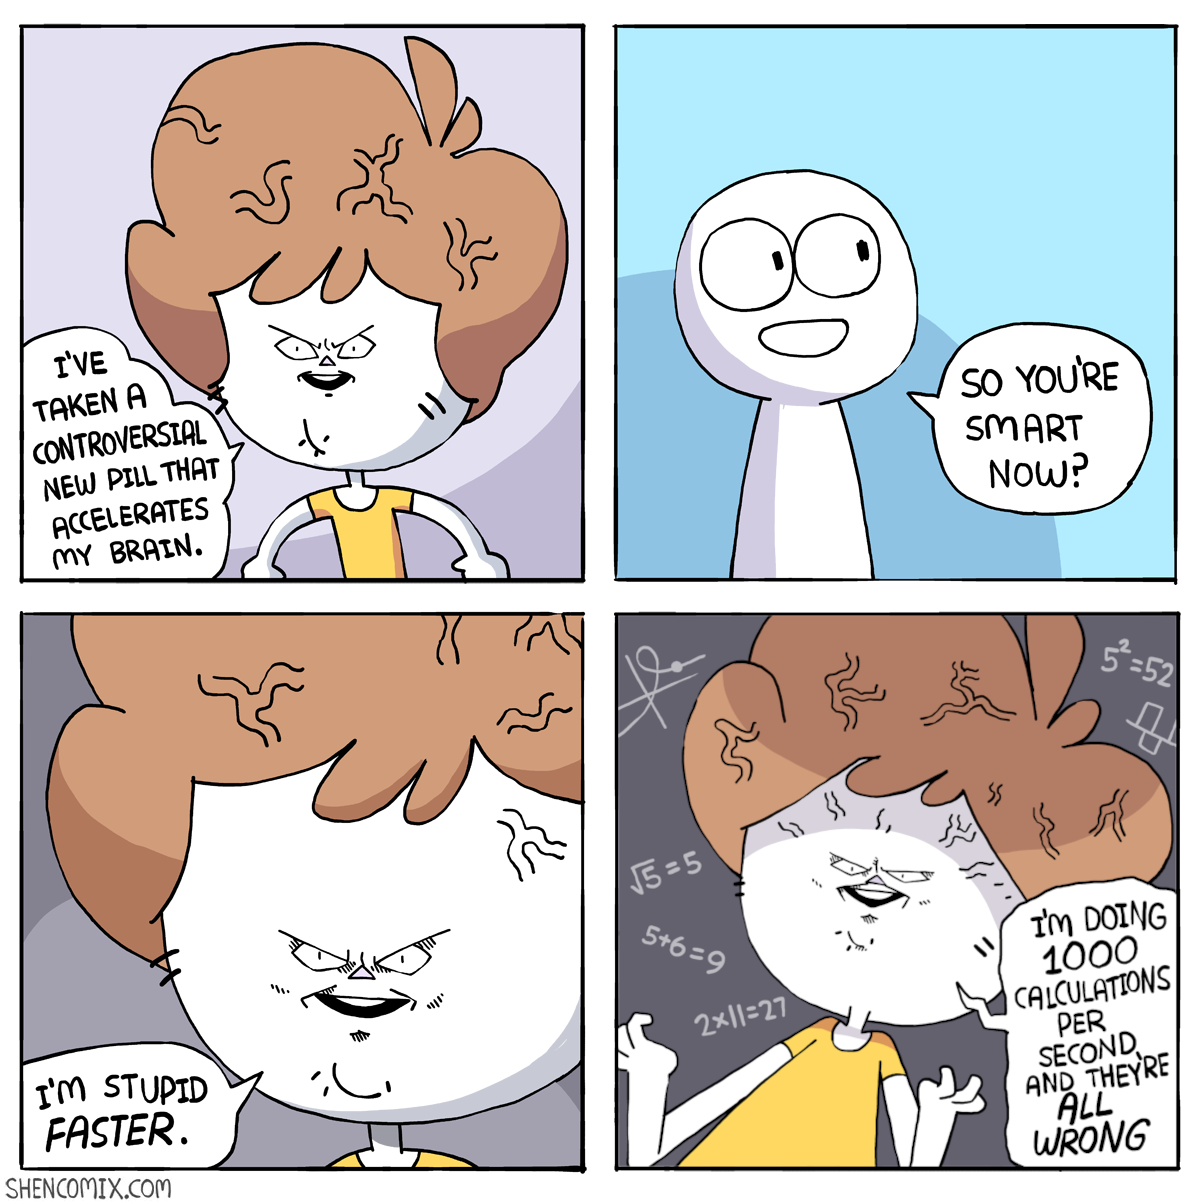
\includegraphics[width=0.75\textwidth]{stupidfaster.png}
    \caption{Stupid Faster \cite{stupidfaster1, stupidfaster2}}\label{stupidfaster}
\end{figure}

\subsection{\MINIROCKET}

\MINIROCKET, fully \emph{\textbf{MINI}mally \textbf{R}and\textbf{O}m \textbf{C}onvolutional \textbf{KE}rnel \textbf{T}ransform}, focuses on removing randomness from the \ROCKET algorithm, while reducing the processing time even further. Instead of generating thousands kernels, \MINIROCKET uses a fixed set of 84 kernel weights (as proven in Theorem \ref{proof_kernel_84}) of length  9, built purely from six values of -1 and three values of 2.

\begin{theorem}
\label{proof_kernel_84}
There are 84 kernel weights combinations used in \MINIROCKET.

\begin{proof}
    Let 9 be the length of the kernel and 6 be the number of values set to -1 and 3 be the number of values set to 2. Then, by choosing 3 spots in the kernel, we get $\binom{9}{3}=84$ unique kernel weights combinations.
\end{proof}
\end{theorem}

Simply said, the dilation and it's intensity is based on the input length and the number of different dilations per each kernel (combination of -1 and 2) is based on the number of features requested. Padding is enabled (or disabled) for every other feature and bias is based on quantiles of the values calculated in the convolution par of the training step. These quantiles are not random but based on \emph{golden-ratio-modulo-one} series, providing low discrepancy series for the whole $[0, 1]$ interval.

\begin{table}[!h]
    \unuglifytable
    \begin{tabular}{l | c c}
        \hline
                   & \ROCKET              & \MINIROCKET           \\
        \hline
        length     & $\{7, 9, 11\}$       & $9$                   \\
        weight     & $\mathbb{N}(0, 1)$   & $\{-1, 2\}$           \\
        bias       & $\mathbb{U}(-1, 1)$  & based on convolution  \\
        dilatation & random               & fixed                 \\
        padding    & \{yes, no\}          & deterministic         \\
        features   & PPV, MAX             & PPV                   \\
        \hline
    \end{tabular}
    \caption{\ROCKET a \MINIROCKET comparison}\label{tab:rocketvsminirocket}
\end{table}

Thanks to this approach, \MINIROCKET does not even really need to calculate every single of these convolutions, but it can just add $-1$ and $2$-multiples of the input values, shifted by dilation and padding. This means that these multiples can be computed only once for each time series and then reused for every weights-dilation-padding-bias combination. Let $\alpha$ be the $-1$-multiple and $\beta$ the $2$-multiple of the input time series of length $n$. For kernel with dilation 1 and the 2-values in position 2 (and two other), we can construct a matrix $C^\prime$
$$
C^\prime = \left[\begin{array}{ccccccc}
    0        & 0        & 0        & 0        & \alpha_1 & \cdots & \alpha_{n-4} \\
    0        & 0        & 0        & \beta_1  & \beta_2  & \cdots & \beta_{n-3}  \\
    0        & 0        & \alpha_1 & \alpha_2 & \alpha_3 & \cdots & \alpha_{n-2} \\
    \vdots   & \vdots   & \vdots   & \vdots   & \vdots   & \ddots & \vdots       \\
    \alpha_4 & \alpha_5 & \alpha_6 & \alpha_7 & \alpha_8 & \cdots & 0            \\
    \alpha_5 & \alpha_6 & \alpha_7 & \alpha_8 & \alpha_9 & \cdots & 0            \\
\end{array}\right],
$$
which, when columns are summed, is equal to the convolution output. These calculations can be simplified even further. Let $C_\alpha$ be a vector of $C^\prime$ column sums for kernel which is made purely of $-1$-multiples. We can, based on the fact that -1 + 3 = 2, make $C_\gamma$, a vector made out of sum of $2$-multiple rows from $C^\prime$. We can keep $C_\alpha$ for each dilation and re-calculate $C_\gamma$ only based on the location of the thee $2$-multiple rows in $C^\prime$. This way we can get rid of all multiplications in the algorithm (we just need to flip the sign for $\alpha$ and do two additions for $\beta$ in the beginning) and do only $\frac{3}{9}$ sums out of the 9 otherwise required for each weights-dilation combination.

Finally, \MINIROCKET uses only \emph{PPV} as it's pooling function since, according to benchmarks \cite{minirocket} mentioned in the original paper, the classification accuracy decrease is statistically insignificant, while reducing the memory requirements by half and further increasing the performance.

\section{\CUKETA~\texttwemoji{zucchini}}

Introducing \CUKETA~\emjl{zucchini} \footnote{This emoji is based on Twemoji \cite{emoji}, an open-source emoji set created by Twitter.} /sʊketa/, \emph{\textbf{CU}DA accelerated minimally random convolutional \textbf{KE}rnel \textbf{T}r\textbf{A}nsform}. The implementation presented in this project, would not be feasible considering the original implementation of \MINIROCKET. Thanks to inefficient parallelisation and repeated memory allocations (although understandable considering limitations of Python + Numba), the process of conversion to efficient CUDA code would be more challenging and possibly way less efficient thanks to frequent cache misses. Thus, this thesis is based on the implementation that can be found in \footlink{https://github.com/antoninkriz/TimeSeriesClassification.jl}{TimeSeriesClassification.jl} \cite{tscjulia}.

The CUDA implementation is nearly identical, considering the algorithm itself, to the Julia implementation. The main difference is that there are almost no CPU computations. Almost all operations happen on the GPU through multiple CUDA kernels on pure CUDA allocated arrays - no other data structures were required. The exception is the \mintinline{cpp}{fit_dilations} function, which prepares the dilations and calculates the number of final features per dilation.

\subsection{Kernels and their optimisation}

Most CUDA kernels are written in a way to reduce the number of CUDA kernel calls from the host. For example this Julia code:
\begin{minted}{julia}
for idx in 1:(9÷2)
    d = e + dilation * (idx - 1)
    @turbo (@views C[end-d+1:end]) .+= (@views A[begin:d])
end

for idx in (9÷2)+2:9
    d = s + dilation * (idx - ((9 ÷ 2) + 2))
    @turbo (@views C[begin:end-d+1]) .+= (@views A[d:end])
end

for idx in @views INDICES[:, kernel_index]
    if idx < 5
        d = e + dilation * (idx - 1)
        @turbo (@views C[end-d+1:end]) .+= (@views G[begin:d])
    elseif idx > 5
        d = s + dilation * (idx - ((9 ÷ 2) + 2))
        @turbo (@views C[begin:end-d+1]) .+= (@views G[d:end])
    else
        @turbo @views C .+= G
    end
end
\end{minted}
was replaced with just two CUDA kernel calls:
\begin{minted}{cpp}
C_A_add<<<BLOCK_SIZE(input_length, BLOCK_SIZE_C_A)>>>(
    C.get(), A.get(),  input_length, dilation, s, e
);

const auto &[ind0, ind1, ind2] = INDICES[kernel_index];
C_G<<<BLOCK_SIZE(input_length, BLOCK_SIZE_C_G)>>>(
    C.get(), G.get(),  input_length, dilation, s, e,
    ind0, ind1, ind2
);
\end{minted}
and all arithmetic operations and the loops are run on the GPU. The host code is purely managing what operations are being done on the GPU and the GPU in return does not need to do any decision making. \emph{PPV} reductions are done using optimised parallel sum from \cite{nvidiaparallelsumslides}. The reduction leaves some space for more advanced (or rather optimised) reductions, since instead of a recursive reduction, as highlighted in \cite{nvidiaparallelsum}, it uses just \mintinline{cpp}{atomicSum(...)}, which should still be quite fast since we're not using the result of the call. This implementation is therefore balancing performance, readability and my free time.

What could be really optimised is the block size (thread count) for each CUDA kernel. Kernels which are similar (in terms what they do) are using the same block size. This lead to four different block sizes used in the code:\label{sec:blocksizes}
\begin{itemize}
    \item \mintinline{cpp}{BLOCK_SIZE_INIT}\\
        Used for initialising array values from the input time series and generating quantiles from the \emph{golden-ratio-modulo-one} series.
    \item \mintinline{cpp}{BLOCK_SIZE_C_XXX}\\
        Used for operations over the arrays based on the $C^\prime$ matrix, i.e. the \mintinline{cpp}{C_A_add} and \mintinline{cpp}{C_G} CUDA kernels.
    \item \mintinline{cpp}{SIZE_QUANTILE_BIASES}\\
        Used purely for extracting biases based on quantiles in the training phase.
    \item \mintinline{cpp}{BLOCK_SIZE_PPV_PX}\\
        Used for calculating PPV in the transformation phase.
\end{itemize}

To efficiently optimise the block size I used an input of 10 time series with length of 100 000 with randomly generated input data. This is OK, since the algorithm is not dependent on the input values themselves, just the sizes of the input. I compiled the program with each block size being a power of two, ranging from 128 to 1024. This gave me $4^4 = 256$ different versions of the same program. Each version was then ran with its run time averaged over 3 runs. The best results were with following sizes
\begin{itemize}
    \item \mintinline{cpp}{BLOCK_SIZE_INIT} = 512
    \item \mintinline{cpp}{BLOCK_SIZE_C_XXX} = 256
    \item \mintinline{cpp}{SIZE_QUANTILE_BIASES} = 512
    \item \mintinline{cpp}{BLOCK_SIZE_PPV_PX} = 256
\end{itemize}
as can be seen in Attachment \ref{tbl:runtimeperblocksizes}, considering only the run time of the algorithm and ignoring the time of the initial data transfer from the host to the device. This is OK for estimating block sizes since here we care only about the algorithm itself and not the fact that it's running on a GPU.

\subsection{Benchmarks}

Finally we're getting to the part where the CUDA implementation is compared to Python and Julia implementations.
The inputs are randomly generated arrays of dimension $N \times M$ (or rather $M \times N$ in case of column-major arrays in Julia), where $N$ is the number of examples and $M$ is the length of a time series, with following values:
\begin{itemize}
    \item $N = 100, M = 10000$
    \item $N = 100, M = 100000$
    \item $N = 100, M = 1000000$
\end{itemize}
and the test was run 3 times for all values together and the total time (in case of CUDA implementation including the host-to-device transfer time). CUDA version used block sizes from the Section \ref{sec:blocksizes}.

The testing was done on a computer with following hardware and software in the list bellow:
\begin{itemize}
    \item \mintinline{text}{CPU}: Intel i7 11700
    \item \mintinline{text}{GPU}: NVIDIA RTX 3070
    \item \mintinline{text}{RAM}: 80 GB DDR4 3333MHz@CL17
    \item \mintinline{text}{Linux}: Manjaro with Kernel 6.6.26
    \item \mintinline{text}{CUDA}: cuda\_12.3.r12.3/compiler.33567101\_0
    \item \mintinline{text}{Julia}: 1.10.0
    \item \mintinline{text}{TimeSeriesClassification.jl}: 1.0.0
    \item \mintinline{text}{Python}: 3.11.8
    \item \mintinline{text}{sktime}: 0.29.0
    \item \mintinline{text}{numpy}: 1.26.4
    \item \mintinline{text}{numba}: 0.59.1
\end{itemize}

\subsection{Results}

As can be seen on the Table \ref{tab:results} and the Figure \ref{img:results}, the CUDA implementation is much slower for time series of short lengths. This is expected due to the need of repeated CUDA kernel calls, which happen to be much slower than the locally running code, still possibly present in the CPU cache. This difference is even more significant with larger amount of short time series, since non-CUDA implementations can process multiple examples (time series) using multiple threads thanks to multi-threading. On the other hand the CUDA implementation is at least 2 times faster for data of large length since the performance of the GPU relies on parallelisation per the number of observation of each time series.

\begin{table}[!h]
\unuglifytable
\begin{tabular}{l|rrrr}
implementation / time series length     & 10 000                     & 100 000                      & \textbf{1 000 000}                     \\
\hline
\CUKETA~\emjl{zucchini}                  & 1 851                      & \textcolor{VioletRed}{3 274} & \textcolor{VioletRed}{\textbf{27 515}} \\
TimeSeriesClassification.jl - 8 threads & \textcolor{VioletRed}{502} & 4 940                        & \textbf{57 710}                        \\
TimeSeriesClassification.jl - 1 thread  & 918                        & 9 100                        & \textbf{92 917}                        \\
sktime - 8 threads                      & 857                        & 13 082                       & \textbf{314 905}
\end{tabular}
\caption{Run time in milliseconds per implementation and time series length (per 100 examples)}\label{tab:results}
\end{table}

\begin{figure}[!h]
    \begin{tikzpicture}
        \begin{axis}[
            xlabel={Time Series Length},
            xmajorgrids=true,
            xtick={1, 2, 3},
            xticklabels={10 000, 100 000, 1 000 000},
            ylabel={Run Time (ms)},
            ymajorgrids=true,
            yminorgrids=true,
            ymode=log,
            legend pos=north west,
            legend cell align=left,
            grid style=dashed,
            minor grid style={dashed, very thin, lightgray},
            width=11cm,
            height=8cm
        ]
        \addplot[
            draw=ForestGreen,
            fill=ForestGreen,
            mark=square*,
            only marks,
            ]
            coordinates {
            (1,1851)(2,3274)(3,27515)
            };
            \addlegendentry{\CUKETA~\emjl{zucchini}}
    
        \addplot[
            color=Crimson,
            fill=Crimson,
            mark=triangle*,
            only marks,
            ]
            coordinates {
            (1,502)(2,4940)(3,57710)
            };
            \addlegendentry{TimeSeriesClassification.jl - 8 threads}
            
        \addplot[
            color=DodgerBlue,
            fill=DodgerBlue,
            mark=diamond*,
            only marks,
            ]
            coordinates {
            (1,918)(2,9100)(3,92917)
            };
            \addlegendentry{TimeSeriesClassification.jl - 1 thread}
            
        \addplot[
            color=Orange,
            fill=Orange,
            mark=*,
            only marks,
            ]
            coordinates {
            (1,857)(2,13082)(3,314905)
            };
            \addlegendentry{sktime - 8 threads}
    
        \end{axis}
    \end{tikzpicture}
    \caption{Benchmarked run times per implementation and time series length (per 100 examples)}\label{img:results}
\end{figure}

\section{Conclusion}

\CUKETA~\emjl{zucchini}, the CUDA accelerated implementation of \MINIROCKET, performs much better on time series of large lengths, while current implementations benefit from large number of shorter time series. This was expected due to the way each algorithm utilises parallelisation. When time series length is of at least $100\ 000$ observations, \CUKETA~\emjl{zucchini} tends to perform $1.5\times$ faster than the fastest CPU implementation of the \MINIROCKET algorithm and $4\times$ faster than the official implementation. For a time series with $1\ 000\ 000$ observation \CUKETA~\emjl{zucchini} is at least $2\times$ and $11.4\times$ faster respectively.







\newpage
\printbibliography

\newpage
\section{Attachments}

\subsection{Run time per block sizes}
\label{tbl:runtimeperblocksizes}

\begin{itemize}
    \item \mintinline{cpp}{B1} = \mintinline{cpp}{BLOCK_SIZE_INIT}
    \item \mintinline{cpp}{B2} = \mintinline{cpp}{BLOCK_SIZE_C_XXX}
    \item \mintinline{cpp}{B3} = \mintinline{cpp}{SIZE_QUANTILE_BIASES}
    \item \mintinline{cpp}{B4} = \mintinline{cpp}{BLOCK_SIZE_PPV_PX}
    \item \mintinline{cpp}{duration} = run time of the whole algorithm excluding copying data from the host to the device in milliseconds
\end{itemize}

{\footnotesize
\begin{longtable}{rrrrrrr}
\hline
\mintinline{cpp}{B1} & \mintinline{cpp}{B2} & \mintinline{cpp}{B3} & \mintinline{cpp}{B4} & \mintinline{cpp}{duration} \\
\hline\endfirsthead
\hline
\mintinline{cpp}{B1} & \mintinline{cpp}{B2} & \mintinline{cpp}{B3} & \mintinline{cpp}{B4} & \mintinline{cpp}{duration} \\
\hline\endhead
512 & 256 & 512 & 256 & 489.333333 \\
512 & 256 & 1024 & 128 & 490.333333 \\
512 & 128 & 1024 & 256 & 490.666667 \\
256 & 256 & 512 & 128 & 490.666667 \\
512 & 256 & 256 & 256 & 490.666667 \\
512 & 128 & 512 & 128 & 491.000000 \\
256 & 256 & 1024 & 128 & 491.000000 \\
256 & 256 & 128 & 256 & 491.000000 \\
256 & 256 & 1024 & 256 & 491.333333 \\
256 & 256 & 256 & 128 & 491.333333 \\
256 & 256 & 256 & 256 & 491.333333 \\
256 & 256 & 512 & 256 & 491.333333 \\
512 & 256 & 1024 & 256 & 491.666667 \\
512 & 256 & 128 & 128 & 491.666667 \\
512 & 128 & 256 & 128 & 491.666667 \\
512 & 256 & 512 & 128 & 491.666667 \\
256 & 256 & 128 & 128 & 491.666667 \\
512 & 128 & 256 & 256 & 492.000000 \\
256 & 512 & 512 & 256 & 492.333333 \\
512 & 256 & 128 & 256 & 492.333333 \\
512 & 128 & 512 & 256 & 492.333333 \\
512 & 256 & 256 & 128 & 492.666667 \\
512 & 128 & 128 & 256 & 492.666667 \\
512 & 128 & 1024 & 128 & 492.666667 \\
512 & 128 & 128 & 128 & 493.000000 \\
512 & 512 & 256 & 256 & 493.000000 \\
256 & 512 & 128 & 256 & 493.000000 \\
256 & 512 & 1024 & 256 & 493.333333 \\
512 & 512 & 128 & 128 & 493.333333 \\
512 & 512 & 128 & 256 & 493.333333 \\
256 & 512 & 512 & 128 & 493.666667 \\
512 & 512 & 512 & 128 & 493.666667 \\
256 & 512 & 256 & 256 & 493.666667 \\
256 & 512 & 256 & 128 & 494.000000 \\
512 & 512 & 256 & 128 & 494.333333 \\
128 & 256 & 1024 & 256 & 494.333333 \\
256 & 512 & 128 & 128 & 494.333333 \\
128 & 256 & 256 & 256 & 494.666667 \\
128 & 256 & 1024 & 128 & 494.666667 \\
128 & 256 & 512 & 256 & 495.000000 \\
512 & 512 & 512 & 256 & 495.000000 \\
128 & 128 & 1024 & 256 & 495.000000 \\
512 & 512 & 1024 & 256 & 495.333333 \\
128 & 256 & 128 & 256 & 495.333333 \\
256 & 512 & 1024 & 128 & 495.333333 \\
128 & 128 & 512 & 256 & 495.666667 \\
512 & 512 & 1024 & 128 & 495.666667 \\
128 & 128 & 128 & 128 & 495.666667 \\
256 & 128 & 128 & 128 & 495.666667 \\
128 & 256 & 256 & 128 & 496.000000 \\
128 & 256 & 128 & 128 & 496.000000 \\
128 & 128 & 512 & 128 & 496.333333 \\
128 & 512 & 128 & 256 & 496.333333 \\
256 & 128 & 128 & 256 & 496.333333 \\
128 & 128 & 128 & 256 & 496.333333 \\
256 & 128 & 256 & 128 & 496.666667 \\
128 & 128 & 256 & 256 & 496.666667 \\
256 & 128 & 512 & 128 & 496.666667 \\
128 & 128 & 256 & 128 & 497.000000 \\
128 & 512 & 1024 & 256 & 497.000000 \\
256 & 128 & 256 & 256 & 497.000000 \\
256 & 128 & 1024 & 128 & 497.000000 \\
256 & 128 & 1024 & 256 & 497.000000 \\
128 & 128 & 1024 & 128 & 497.333333 \\
1024 & 128 & 1024 & 256 & 497.333333 \\
128 & 512 & 256 & 256 & 497.666667 \\
1024 & 512 & 512 & 256 & 497.666667 \\
1024 & 512 & 256 & 256 & 498.000000 \\
128 & 512 & 128 & 128 & 498.000000 \\
256 & 128 & 512 & 256 & 498.000000 \\
128 & 256 & 512 & 128 & 498.000000 \\
128 & 512 & 512 & 128 & 498.333333 \\
1024 & 256 & 128 & 256 & 498.333333 \\
128 & 512 & 1024 & 128 & 498.333333 \\
128 & 512 & 256 & 128 & 498.333333 \\
1024 & 256 & 256 & 256 & 498.666667 \\
128 & 512 & 512 & 256 & 498.666667 \\
1024 & 128 & 256 & 256 & 498.666667 \\
1024 & 512 & 512 & 128 & 499.000000 \\
1024 & 128 & 128 & 128 & 499.000000 \\
1024 & 128 & 1024 & 128 & 499.333333 \\
1024 & 256 & 1024 & 256 & 499.666667 \\
1024 & 256 & 512 & 256 & 499.666667 \\
1024 & 128 & 128 & 256 & 499.666667 \\
1024 & 512 & 256 & 128 & 500.000000 \\
1024 & 256 & 256 & 128 & 500.000000 \\
1024 & 256 & 1024 & 128 & 500.333333 \\
1024 & 256 & 128 & 128 & 500.333333 \\
1024 & 128 & 512 & 256 & 500.666667 \\
1024 & 512 & 128 & 256 & 501.333333 \\
1024 & 128 & 512 & 128 & 501.333333 \\
1024 & 256 & 512 & 128 & 502.000000 \\
1024 & 128 & 256 & 128 & 502.000000 \\
1024 & 512 & 1024 & 256 & 502.333333 \\
1024 & 512 & 1024 & 128 & 503.000000 \\
1024 & 512 & 128 & 128 & 503.333333 \\
512 & 1024 & 1024 & 256 & 510.000000 \\
512 & 1024 & 512 & 256 & 510.333333 \\
1024 & 1024 & 1024 & 128 & 510.666667 \\
512 & 1024 & 256 & 256 & 511.666667 \\
512 & 1024 & 1024 & 128 & 511.666667 \\
512 & 1024 & 128 & 256 & 511.666667 \\
1024 & 1024 & 1024 & 256 & 511.666667 \\
512 & 1024 & 256 & 128 & 512.333333 \\
512 & 1024 & 128 & 128 & 512.666667 \\
1024 & 1024 & 128 & 128 & 513.000000 \\
1024 & 1024 & 128 & 256 & 513.000000 \\
512 & 1024 & 512 & 128 & 514.000000 \\
256 & 1024 & 128 & 256 & 514.000000 \\
256 & 1024 & 256 & 256 & 514.666667 \\
128 & 1024 & 256 & 256 & 514.666667 \\
256 & 1024 & 512 & 128 & 514.666667 \\
128 & 1024 & 128 & 256 & 514.666667 \\
128 & 1024 & 1024 & 256 & 514.666667 \\
256 & 1024 & 128 & 128 & 515.000000 \\
256 & 1024 & 1024 & 256 & 515.000000 \\
256 & 1024 & 512 & 256 & 515.000000 \\
128 & 1024 & 512 & 256 & 515.000000 \\
256 & 1024 & 256 & 128 & 515.333333 \\
256 & 1024 & 1024 & 128 & 515.666667 \\
128 & 1024 & 128 & 128 & 515.666667 \\
128 & 1024 & 256 & 128 & 515.666667 \\
128 & 1024 & 512 & 128 & 516.000000 \\
128 & 1024 & 1024 & 128 & 516.000000 \\
1024 & 1024 & 256 & 128 & 516.333333 \\
1024 & 1024 & 512 & 256 & 517.000000 \\
1024 & 1024 & 256 & 256 & 517.333333 \\
1024 & 1024 & 512 & 128 & 518.333333 \\
256 & 256 & 512 & 512 & 533.333333 \\
512 & 256 & 256 & 512 & 534.000000 \\
256 & 256 & 1024 & 512 & 534.666667 \\
512 & 256 & 128 & 512 & 534.666667 \\
256 & 256 & 128 & 512 & 535.000000 \\
512 & 128 & 1024 & 512 & 535.333333 \\
512 & 256 & 512 & 512 & 535.333333 \\
512 & 256 & 1024 & 512 & 535.666667 \\
512 & 128 & 128 & 512 & 535.666667 \\
512 & 512 & 128 & 512 & 536.000000 \\
256 & 256 & 256 & 512 & 536.000000 \\
256 & 512 & 512 & 512 & 536.000000 \\
512 & 128 & 512 & 512 & 536.000000 \\
512 & 128 & 256 & 512 & 536.333333 \\
256 & 512 & 256 & 512 & 536.666667 \\
256 & 128 & 512 & 512 & 536.666667 \\
256 & 512 & 128 & 512 & 537.000000 \\
512 & 512 & 1024 & 512 & 538.000000 \\
128 & 256 & 128 & 512 & 538.000000 \\
512 & 512 & 512 & 512 & 538.000000 \\
256 & 512 & 1024 & 512 & 538.333333 \\
256 & 128 & 1024 & 512 & 538.666667 \\
128 & 256 & 256 & 512 & 539.000000 \\
128 & 128 & 512 & 512 & 539.000000 \\
128 & 128 & 256 & 512 & 539.333333 \\
512 & 512 & 256 & 512 & 539.333333 \\
128 & 256 & 512 & 512 & 539.333333 \\
128 & 128 & 1024 & 512 & 539.333333 \\
256 & 128 & 256 & 512 & 539.666667 \\
128 & 256 & 1024 & 512 & 539.666667 \\
256 & 128 & 128 & 512 & 539.666667 \\
128 & 128 & 128 & 512 & 540.000000 \\
128 & 512 & 1024 & 512 & 540.666667 \\
128 & 512 & 128 & 512 & 541.000000 \\
1024 & 512 & 256 & 512 & 542.000000 \\
128 & 512 & 512 & 512 & 542.333333 \\
1024 & 512 & 512 & 512 & 542.333333 \\
1024 & 128 & 1024 & 512 & 542.333333 \\
128 & 512 & 256 & 512 & 542.666667 \\
1024 & 256 & 128 & 512 & 542.666667 \\
1024 & 256 & 512 & 512 & 542.666667 \\
1024 & 256 & 1024 & 512 & 543.000000 \\
1024 & 128 & 256 & 512 & 543.666667 \\
1024 & 128 & 512 & 512 & 544.000000 \\
1024 & 128 & 128 & 512 & 544.000000 \\
1024 & 256 & 256 & 512 & 544.333333 \\
1024 & 512 & 128 & 512 & 545.333333 \\
1024 & 512 & 1024 & 512 & 546.333333 \\
512 & 1024 & 1024 & 512 & 554.333333 \\
512 & 1024 & 512 & 512 & 554.666667 \\
512 & 1024 & 256 & 512 & 555.000000 \\
512 & 1024 & 128 & 512 & 555.333333 \\
128 & 1024 & 128 & 512 & 556.333333 \\
1024 & 1024 & 1024 & 512 & 556.333333 \\
128 & 1024 & 256 & 512 & 557.333333 \\
128 & 1024 & 1024 & 512 & 558.000000 \\
256 & 1024 & 128 & 512 & 558.666667 \\
256 & 1024 & 1024 & 512 & 558.666667 \\
128 & 1024 & 512 & 512 & 558.666667 \\
256 & 1024 & 512 & 512 & 558.666667 \\
256 & 1024 & 256 & 512 & 559.000000 \\
1024 & 1024 & 128 & 512 & 559.666667 \\
1024 & 1024 & 256 & 512 & 560.333333 \\
1024 & 1024 & 512 & 512 & 560.666667 \\
256 & 256 & 128 & 1024 & 678.000000 \\
512 & 256 & 256 & 1024 & 678.666667 \\
512 & 256 & 128 & 1024 & 678.666667 \\
256 & 256 & 512 & 1024 & 679.333333 \\
512 & 256 & 1024 & 1024 & 679.666667 \\
512 & 256 & 512 & 1024 & 680.333333 \\
256 & 256 & 256 & 1024 & 680.333333 \\
512 & 128 & 512 & 1024 & 680.666667 \\
256 & 256 & 1024 & 1024 & 680.666667 \\
512 & 128 & 128 & 1024 & 680.666667 \\
512 & 512 & 1024 & 1024 & 681.333333 \\
256 & 512 & 128 & 1024 & 681.333333 \\
512 & 512 & 128 & 1024 & 681.666667 \\
512 & 128 & 1024 & 1024 & 681.666667 \\
512 & 128 & 256 & 1024 & 682.000000 \\
512 & 512 & 512 & 1024 & 682.000000 \\
256 & 512 & 256 & 1024 & 682.333333 \\
256 & 512 & 1024 & 1024 & 683.000000 \\
128 & 128 & 512 & 1024 & 683.666667 \\
128 & 256 & 512 & 1024 & 683.666667 \\
512 & 512 & 256 & 1024 & 683.666667 \\
256 & 512 & 512 & 1024 & 683.666667 \\
128 & 256 & 128 & 1024 & 684.000000 \\
256 & 128 & 128 & 1024 & 684.000000 \\
128 & 128 & 128 & 1024 & 684.666667 \\
128 & 256 & 256 & 1024 & 684.666667 \\
128 & 256 & 1024 & 1024 & 684.666667 \\
128 & 128 & 256 & 1024 & 684.666667 \\
128 & 128 & 1024 & 1024 & 685.000000 \\
256 & 128 & 512 & 1024 & 685.000000 \\
256 & 128 & 1024 & 1024 & 685.666667 \\
128 & 512 & 256 & 1024 & 686.333333 \\
256 & 128 & 256 & 1024 & 686.333333 \\
128 & 512 & 512 & 1024 & 686.666667 \\
128 & 512 & 1024 & 1024 & 686.666667 \\
1024 & 128 & 1024 & 1024 & 687.000000 \\
1024 & 128 & 128 & 1024 & 687.333333 \\
1024 & 512 & 512 & 1024 & 687.666667 \\
128 & 512 & 128 & 1024 & 687.666667 \\
1024 & 256 & 1024 & 1024 & 689.666667 \\
1024 & 256 & 256 & 1024 & 689.666667 \\
1024 & 256 & 128 & 1024 & 689.666667 \\
1024 & 256 & 512 & 1024 & 690.000000 \\
1024 & 128 & 512 & 1024 & 690.333333 \\
1024 & 128 & 256 & 1024 & 691.000000 \\
1024 & 512 & 1024 & 1024 & 691.666667 \\
1024 & 512 & 128 & 1024 & 692.000000 \\
1024 & 512 & 256 & 1024 & 692.333333 \\
512 & 1024 & 256 & 1024 & 698.333333 \\
512 & 1024 & 1024 & 1024 & 698.666667 \\
1024 & 1024 & 128 & 1024 & 699.666667 \\
512 & 1024 & 512 & 1024 & 700.000000 \\
512 & 1024 & 128 & 1024 & 700.666667 \\
256 & 1024 & 1024 & 1024 & 701.333333 \\
128 & 1024 & 256 & 1024 & 702.333333 \\
128 & 1024 & 512 & 1024 & 703.333333 \\
256 & 1024 & 512 & 1024 & 703.333333 \\
128 & 1024 & 1024 & 1024 & 703.333333 \\
256 & 1024 & 128 & 1024 & 704.000000 \\
256 & 1024 & 256 & 1024 & 704.333333 \\
128 & 1024 & 128 & 1024 & 704.666667 \\
1024 & 1024 & 256 & 1024 & 705.000000 \\
1024 & 1024 & 512 & 1024 & 706.000000 \\
1024 & 1024 & 1024 & 1024 & 748.333333 \\
\end{longtable}
}

\end{document}
